\section{Laboratory Lecture 1: VHDL}

In this lab lecture we will design a logic circuit that will act as an interface between the output of an ADC, a 4-bit value, and an array of LEDs so as to represent said value in a visual manner.\medskip

To better understand the circuit that we will be working with, we will start by drawing a simple diagram:\medskip

\begin{figure}[H]
    \centering
    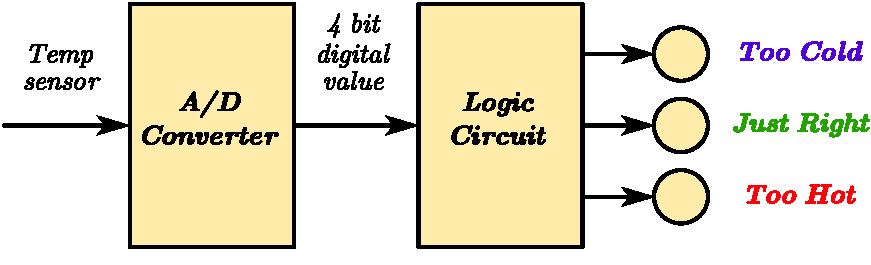
\includegraphics[width=\linewidth]{Graphics/Practice 1/Temp_ADC_Logic.pdf}
    \caption{Circuit block representation.}
    \label{fig:tempcircuit}
\end{figure}

As we can see in the diagram, there is a temperature sensor which output is fed into an analog-to-digital converter. The latter outputs a 4 bit digital value which serves as input to the logic circuit that we have to design. This circuit will interpret the  data and, based on it, it will turn on a specific LED to indicate the temperature range that the sensor is measuring, being these states the ones indicated in the diagram\medskip

To aid the design process, a table containing the possible output values of the ADC and their corresponding meaning is given:

\begin{table}[ht]
    \centering
        \begin{tabular}[t]{lcc}
            \toprule
            &\textbf{Digital Values}&\textbf{Category}\\
            \midrule
            &0000-1000&Too cold\\
            &1001-1010&Just right\\
            &1011-1111&Too hot\\
            \bottomrule
        \end{tabular}
        \caption{Possible states.}
\end{table}

Our job will consist in programming the logic circuit in order to obtain the desired behaviour. In this practice, as well as in the rest of the subject, we will make use of the GAL22V10. This IC, commonly found in the DIP package, though old, is still a very good choice for beginners, due to its simplicity and ease of use.\medskip

\newpage

To program the circuit, we will use the proprietary software designed for it, IspLever Classic. This program will allow us to synthesize and implement our VHDL code into the GAL SPLD. The main advantage of PLDs and FPGAs is the ability to program, using code, the HARDWARE part of our circuit, allowing us to obtain higher switching speeds and a faster response compared to what we would obtain if we were to use a microcontroller.\medskip

Writing some pseudocode before programming our circuit will surely come in handy later, as it is a nice way of organising the code and its different parts.

For this simple case, we came up with the following:\medskip

\begin{algorithm}
        \begin{algorithmic}
            \IF{digital value $\leq 8$}
            \STATE light only the \textcolor{blue}{Too Cold} indicator.
            \ELSIF{8 < digital value < 11}
            \STATE light only the \textcolor{green}{Just Right} indicator.
            \ELSE{}
            \STATE light only the \textcolor{red}{Too Hot} indicator.
            \ENDIF
        \end{algorithmic}
\end{algorithm}

Before starting programming our circuit, we will first define the basic parts of any VHDL program:

\subsection{Library}

One of the most important parts of any VHDL program is the inclusion of several, important libraries.\textbf{Libraries} are pre-written chunks of code that allow us to focus on the development of our code without having to worry too much about the technical and laborious parts of the language itself.

The structure of this part is as follows:

\begin{code}{vhdl}
library ieee;
use ieee.std_logic_1164.all;
use ieee.std_logic_arith.all;
use ieee.std_logic_unsigned.all;
\end{code}

Here we can find a library clause, for instance, \textbf{library ieee;} , and a use clause, \textbf{use ieee.std\textunderscore logic\textunderscore 1164.all;}, among others. This gives the code access to all the names declared within package \textbf{std\textunderscore logic\textunderscore 1164} in the library \textbf{ieee}, and to data type \textbf{std\textunderscore logic} in particular.\medskip

We can include other libraries such as \textbf{ieee.std\textunderscore logic\textunderscore arith} which defines some types and basic arithmetic operations for representing integers in standard ways.

\newpage

\subsection{Entity}

An \textbf{entity} can be though of as a black box with inputs and outputs. The entity declaration includes the \textbf{name} of the entity, and a set of port declarations. A \textbf{port} may correspond to a pin on an IC, an edge connector on a board, or any logical channel of communication with a block of hardware.\medskip

Each port declaration includes the \textbf{name of one or more ports}, the \textbf{direction} that information is allowed to flow through the ports \textbf{(in, out or inout)}, and the data type of the ports (i.e., \textbf{std\textunderscore logic}). \medskip

The structure of this part is as follows:

\begin{code}{vhdl}
entity NAME_ENTITY is
  port(NAME_OF_PORT_1:  DIRECTION  DATA_TYPE;
                      . . .
       );
end NAME_ENTITY;
\end{code}

\subsection{Architecture}

The \textbf{architecture} is no longer a definition of parameters but the code itself. The architecture describes the design and is bounded to the entity. 

The syntax for VHDL architecture is as follows: 

\begin{code}{vhdl}
architecture ARCH of NAME_ENTITY is
--begin
--  process(sensitivity list)
  begin
    concurrent/sequential instructions
end ARCH;
\end{code}

In VHDL, it is possible to find more than one architecture. Depending on the complexity of the actions that need to be performed by the PLD/FPGA, we may use concurrent statements, sequential ones -with \textbf{processes}-, or both.\medskip

The architecture has two parts. The declaration part, between the keywords \textbf{\textit{architecture}} and \textbf{\textit{begin}}, in which the interconnection signals, other components referenced by this architecture, or constants are defined and a second part, which starts after the keyword \textbf{\textit{begin}} that includes the statements and assignments and structure of the design.

\newpage

Now that every part of the code has been tacked, we will write the actual code that we will program into the GAL:

\begin{code}{vhdl}
library ieee;
use ieee.std_logic_1164.all;
use ieee.std_logic_arith.all;
use ieee.std_logic_unsigned.all;

entity TEMP is
  port(temp: in std_logic_vector (3 downto 0);
       blue: out std_logic;
       green: out std_logic;  
       red: out std_logic
      );
end TEMP;

architecture SENSOR of TEMP is
  begin
    compare: process(temp)
      begin
      
        if(temp <= "1000") then
          blue <= '1';
          green <= '0';
          red <= '0';
          
          elsif(temp >= "1001" AND temp <= "1010") then
            blue <= '0';
            green <= '1';
            red <= '0';
            
            else
              blue <= '0';
              green <= '0';
              red <= '1';
              
        end if;
    end process;		
end SENSOR;
\end{code}

\newpage

In order to fully understand the code, we will break it down into small chunks.

\begin{code}{vhdl}
entity TEMP is
  port(temp: in std_logic_vector (3 downto 0);
       blue: out std_logic;
       green: out std_logic;  
       red: out std_logic
      );
end TEMP;
\end{code}

As indicated in Figure \ref{fig:tempcircuit}, we will make use of 4 inputs, tied together in a vector, and 3 outputs, which will be connected to our LEDs. This concludes the entity part of our code.

Now, we will analyse its architecture:

\begin{code}{vhdl}
architecture SENSOR of TEMP is
  begin
    compare: process(temp)
      begin
      
        if(temp <= "1000") then
          blue <= '1';
          green <= '0';
          red <= '0';
          
          elsif(temp >= "1001" AND temp <= "1010") then
            blue <= '0';
            green <= '1';
            red <= '0';
            
            else
              blue <= '0';
              green <= '0';
              red <= '1';
              
        end if;
    end process;		
end SENSOR;
\end{code}

As we can see, this architecture is sequential, i.e. the statements don't occur at the same time but one after the other. This is illustrated in line 3, in which the keyword \textbf{process} and a sensitivity list containing the vector \textbf{temp} are introduced. Every time that the value of \textbf{temp} changes, the code linked to that process is run. In our case, this code checks the value of the temperature and turns one of the three LEDs on based on the reading.

\newpage

After programming the code, it is time to compile it using \textbf{IspLeverClassic}. To do this, we will click on \textbf{Create Fuse Map} and wait for it to finish. Once compiled, we will flash the JEDEC file, which contains the fuse arrangement, into the GAL. The set up process won't be included into the reports as it is quite long and not really worth the explanation.\medskip

\begin{figure}[H]
    \centering
    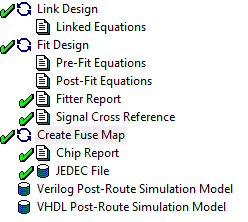
\includegraphics[scale = 0.85]{Graphics/Practice 1/ISPLever.PNG}
    \caption{ISPLever.}
    \label{fig:ISPLever}
\end{figure}

Due to the simplicity of the GAL, the pin assignments are automatically performed by the software, so we have to check which pins the compiler decided to use. To do this, we will make use of the \textbf{Chip Report} pop-up menu.

\begin{figure}[H]
    \centering
    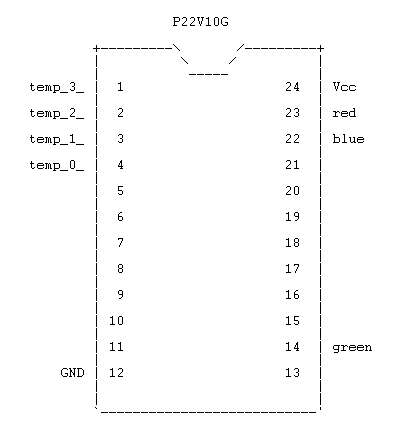
\includegraphics[scale=0.7]{Graphics/Practice 1/Chip_Report.PNG}
    \caption{Chip Report Output.}
    \label{fig:CHIP_REPORT}
\end{figure}

\newpage

Once everything checks, we will move on to simulating the circuit before finally assembling it. To do this, we will make use of ISIS Proteus, a well-know electronics simulation software.\medskip

Knowing the pin assignments makes the task of simulating the circuit very simple, as the only thing required is to follow the \textbf{Chip Report's} connections in Proteus.

\begin{figure}[H]
    \centering
    
    \ifnum\value{ANIMATION}=1 {
        \animategraphics[controls,loop,scale=1.2]{2}{Graphics/Practice 1/ANIMATION/F}{0}{15}
    } 
    \else {
        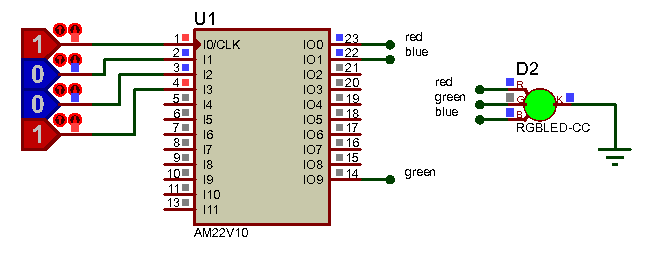
\includegraphics[scale=1.2]{Graphics/Practice 1/ANIMATION/F9.PDF}
    }\fi
    
    \caption{Proteus assembly.}
    \label{fig:PROTEUS_TEMP}
\end{figure}

Now that we have checked that the circuit works as intended, we can proceed to the real assembly. Again, this is just a matter of following the previous connections but this time using a protoboard and some hook-up wires. \medskip

As expected, everything worked great.

\newpage